% !TeX root = ../main.tex

\chapter{蒙特卡罗模拟}
\label{chap:Simulation}

氚衰变 $\beta$ 能谱如图 \ref{fig:eSpectrum} 所示。

\begin{figure}[htbp]
	\centering
	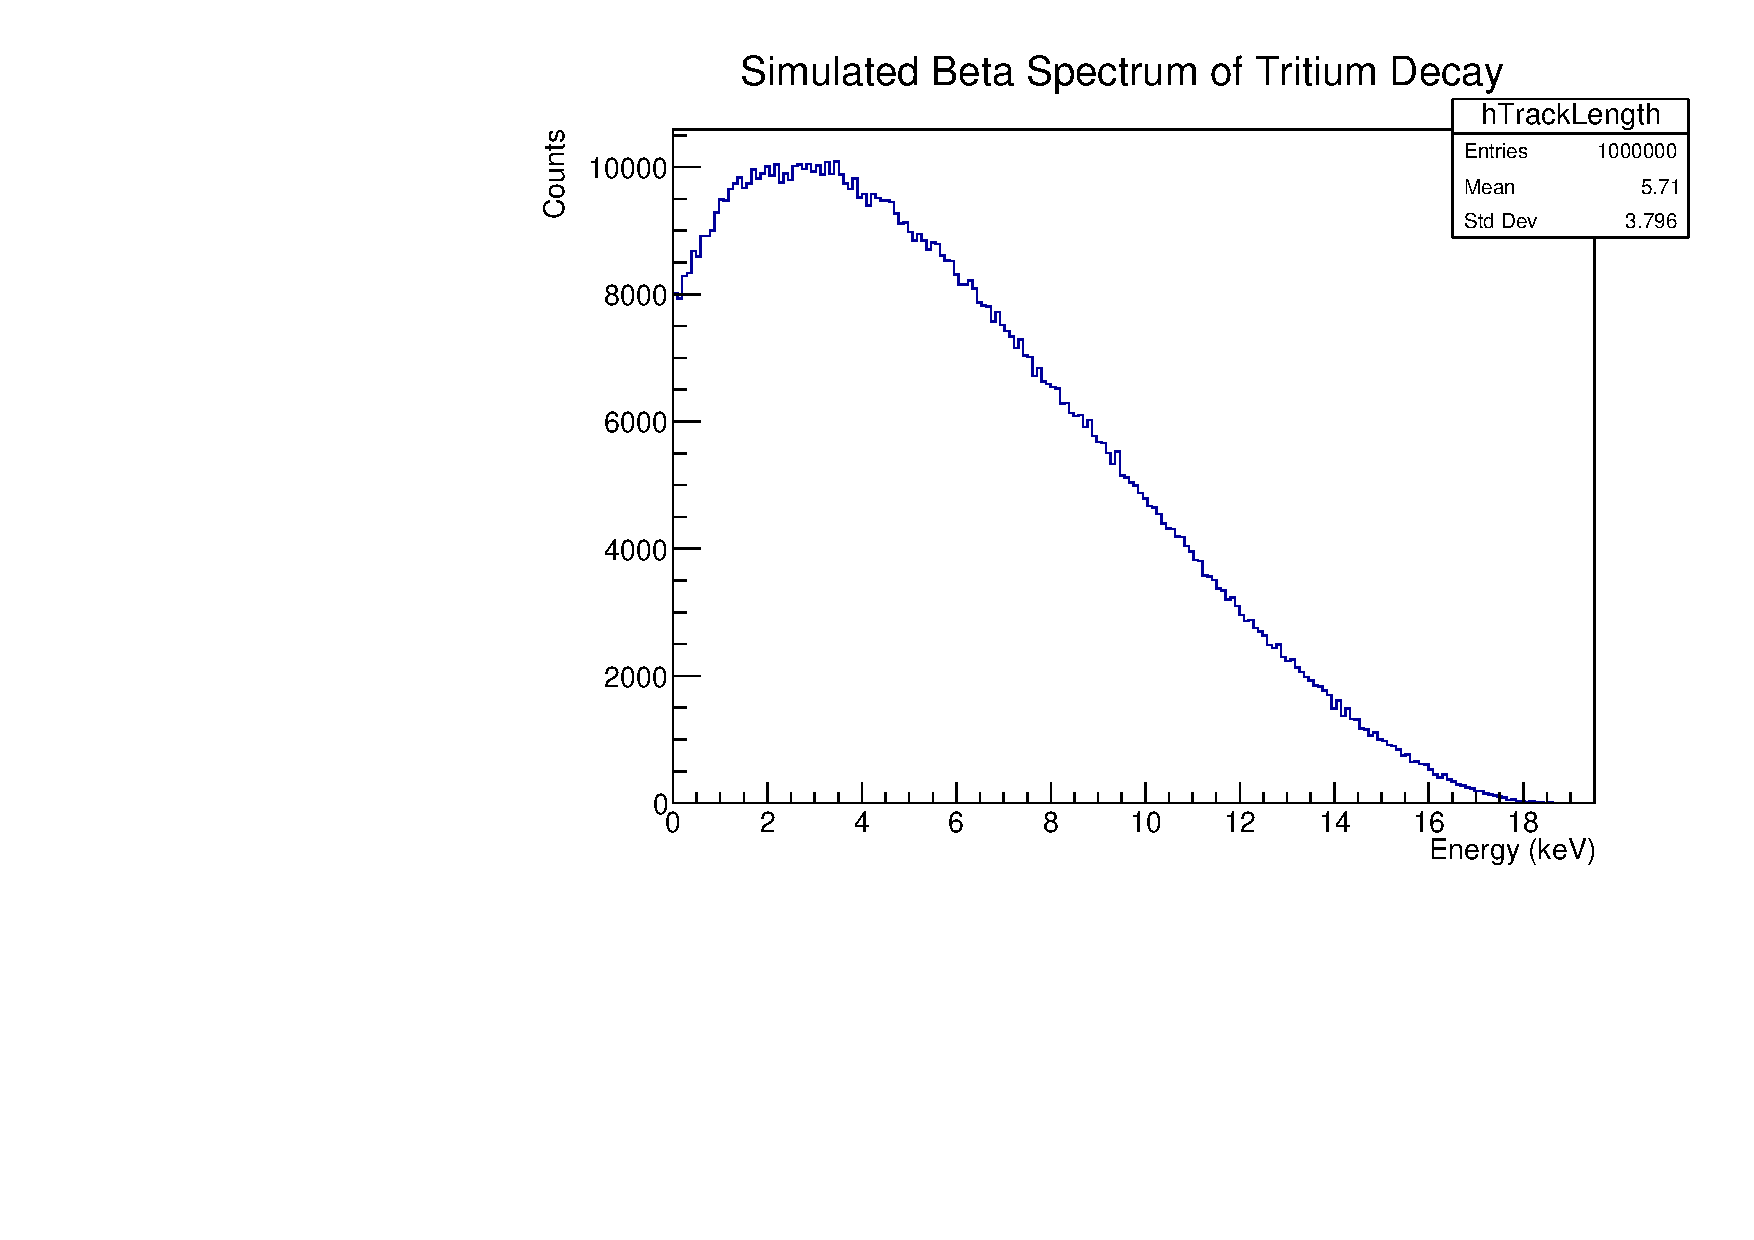
\includegraphics[width=0.8\textwidth]{figures/eSpectrum.pdf}
	\caption{氚衰变 $\beta$ 能谱}
	\label{fig:eSpectrum}
\end{figure}

\section{氚衰变 $\beta$ 在不同材料中的射程}

\begin{figure}[htbp]
	\centering
	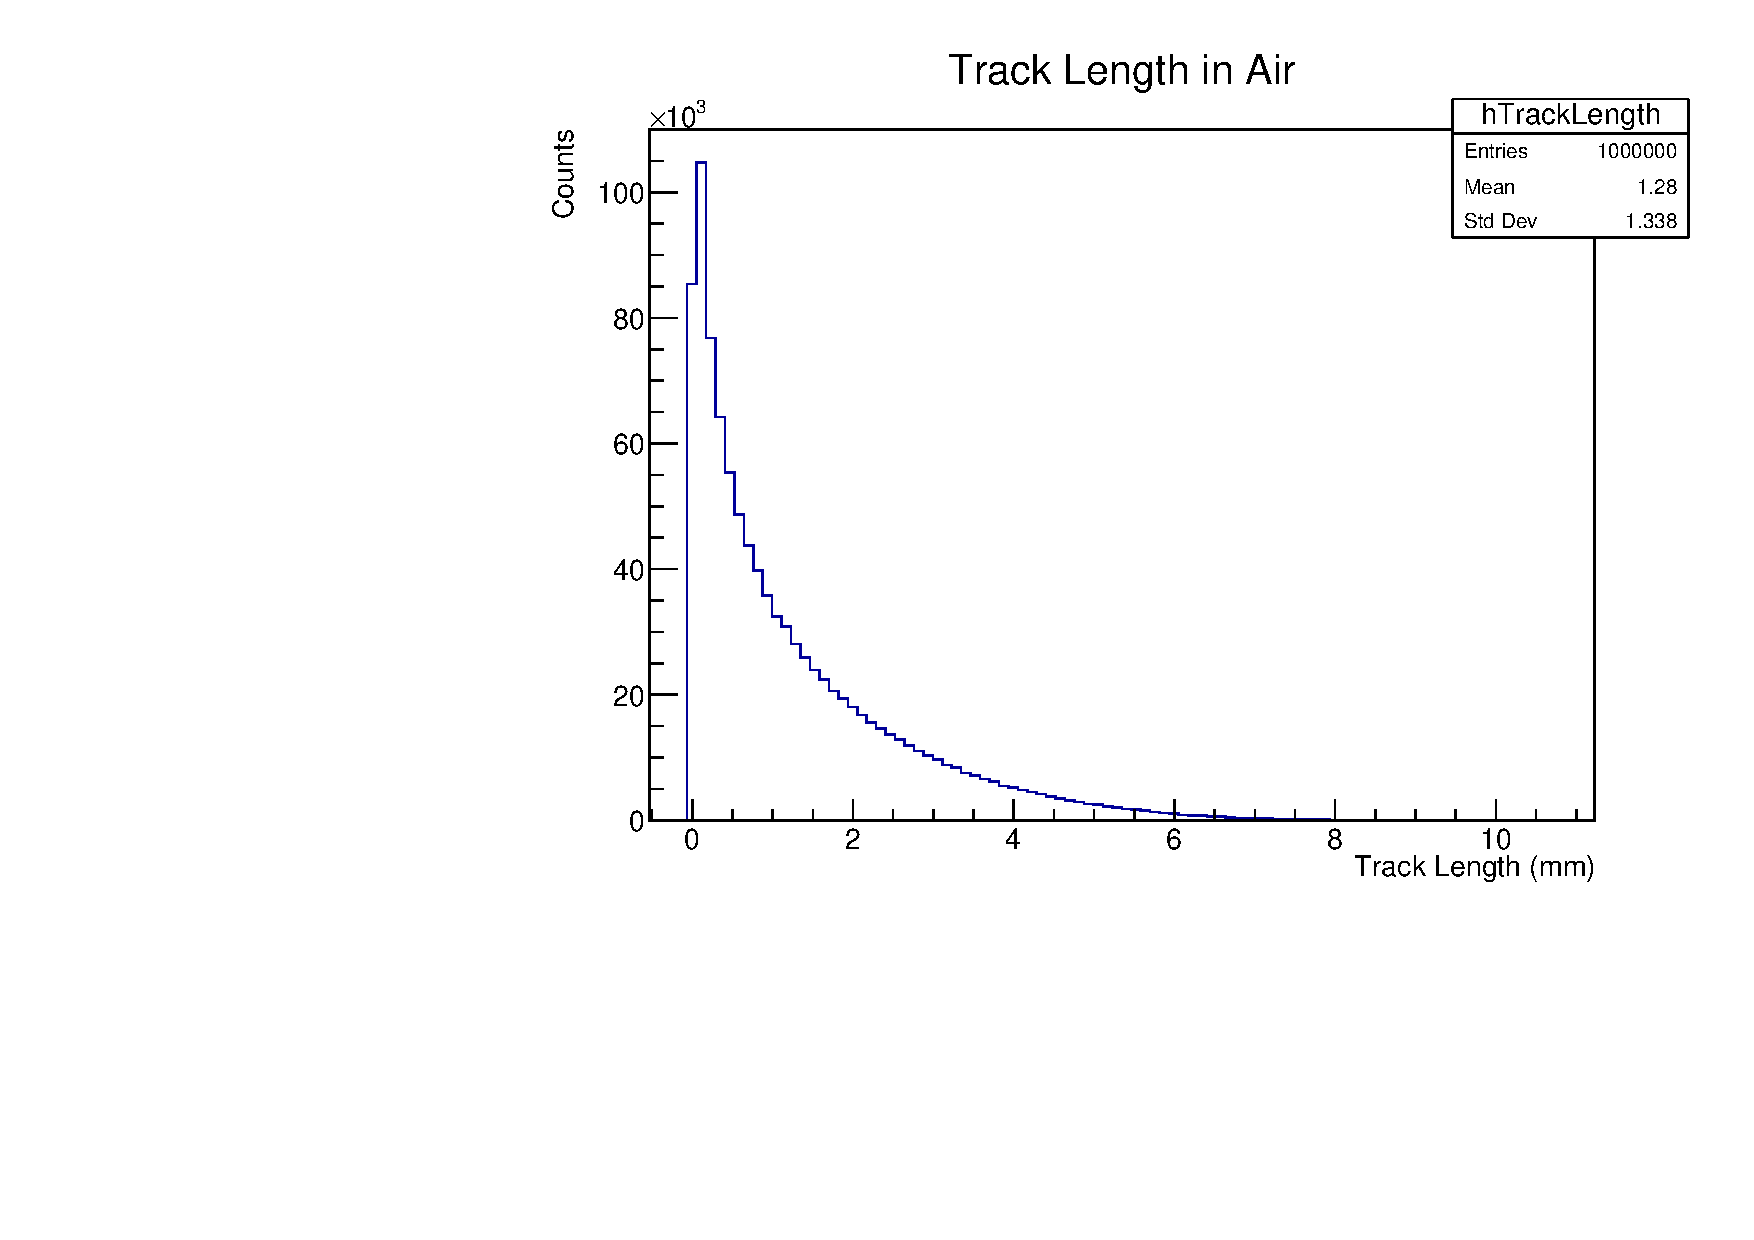
\includegraphics[width=0.8\textwidth]{figures/AirTrackLength.pdf}
	\caption{氚衰变 $\beta$ 在空气中的射程}
	\label{fig:AirTrackLength}
\end{figure}

\begin{figure}[htbp]
	\centering
	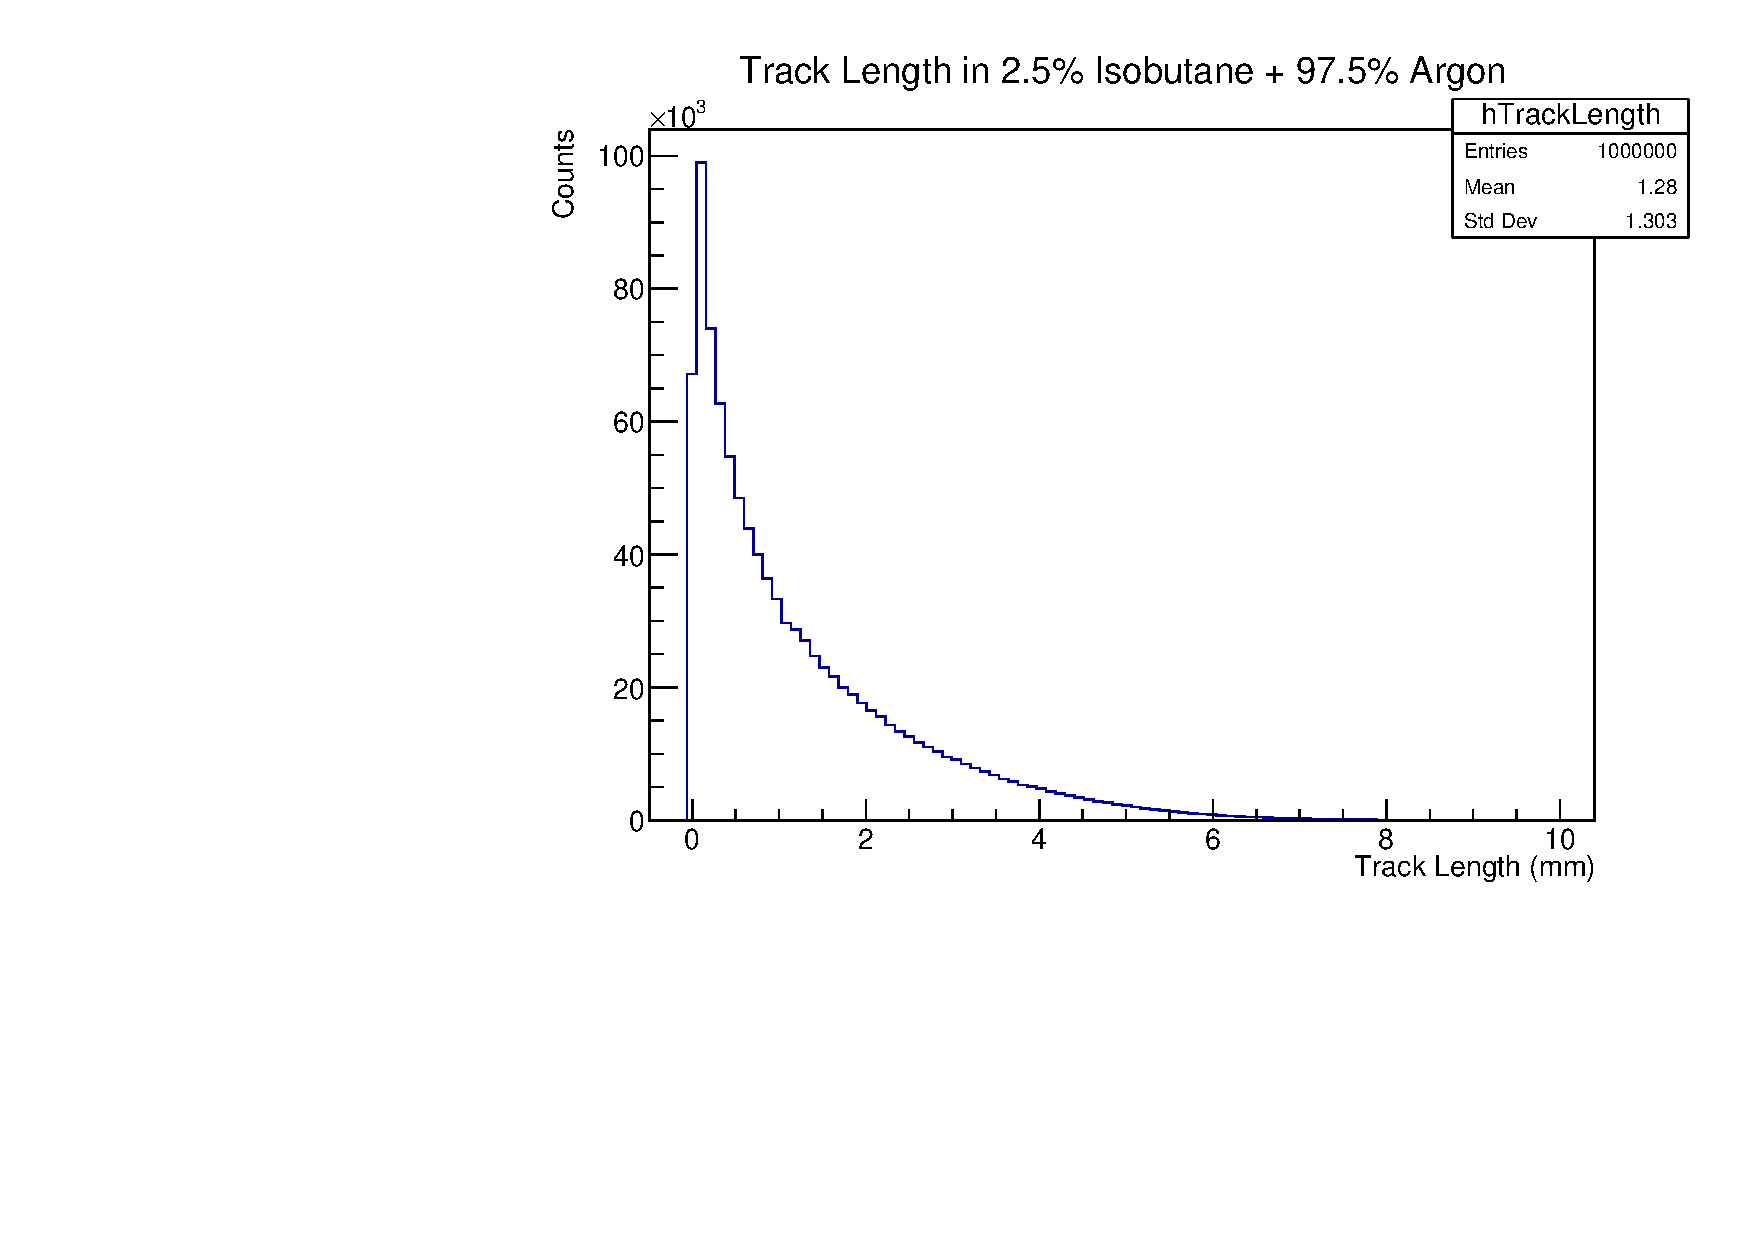
\includegraphics[width=0.8\textwidth]{figures/ArC4H10TrackLength.pdf}
	\caption{氚衰变 $\beta$ 在 97.5\% 氩气和 2.5\% 异丁烷中的射程}
	\label{fig:ArC4H10TrackLength}
\end{figure}

\begin{figure}[htbp]
	\centering
	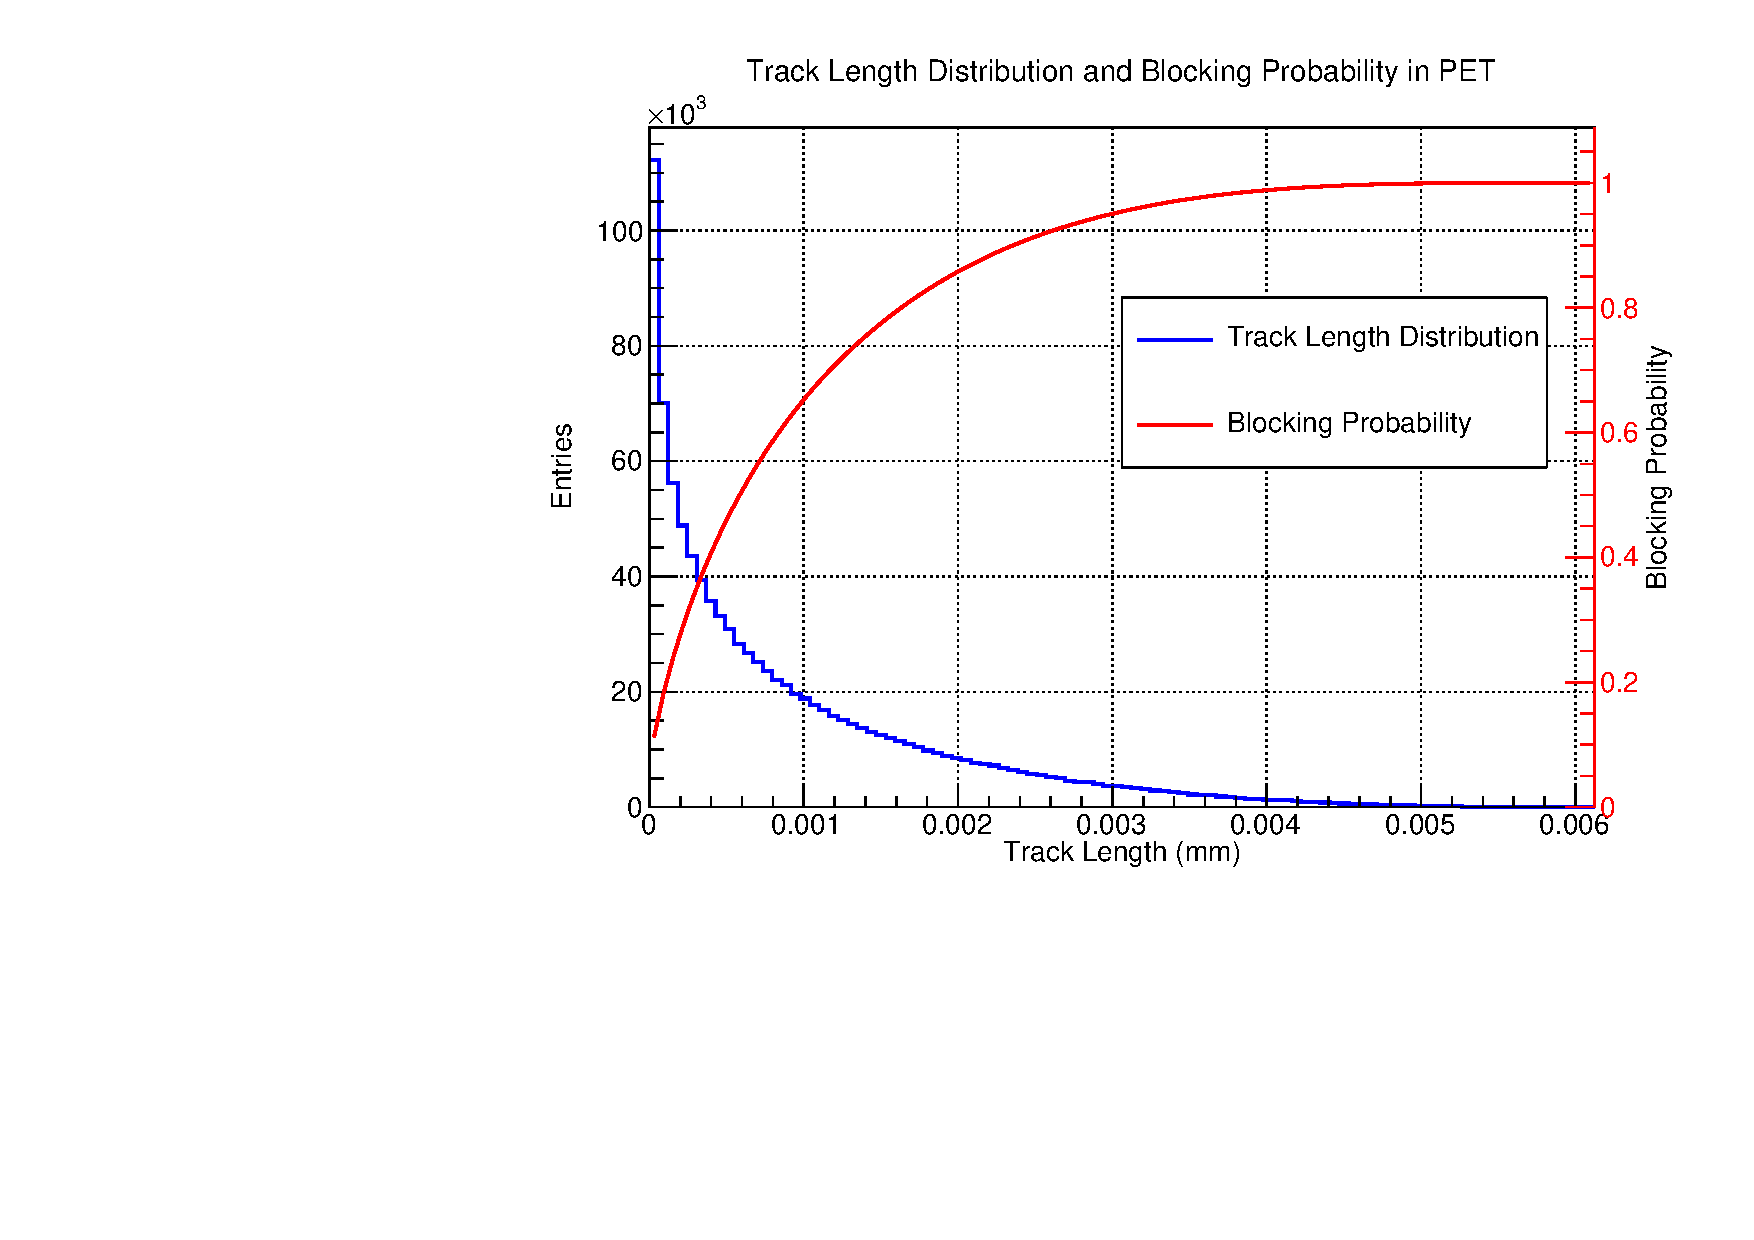
\includegraphics[width=0.8\textwidth]{figures/PETTrackLength.pdf}
	\caption{氚衰变 $\beta$ 在 PET 材料中的射程($\beta$ 粒子垂直入射 PET 材料,统计径迹的总路程;蓝线表示 $\beta$ 径迹总路程在对应区间内的事例数;红线表示 $\beta$ 粒子走过对应径迹长度时被完全吸收的事例占总事例的比重)}
	\label{fig:PETTrackLength}
\end{figure}

\section{氚衰变 $\beta$ 穿透不同厚度的 PET 材料后在氩气中沉积的能谱}

将氚均匀分布在膜窗的一面上,使其衰变,每次运行发射了 1000000 个氚衰变 $\beta$ 粒子,并记录其穿透 PET 材料后在氩气中沉积的能谱,模型如图 \ref{fig:TritiumBetaPenetratePET} 所示。

\begin{figure}[htbp]
	\centering
	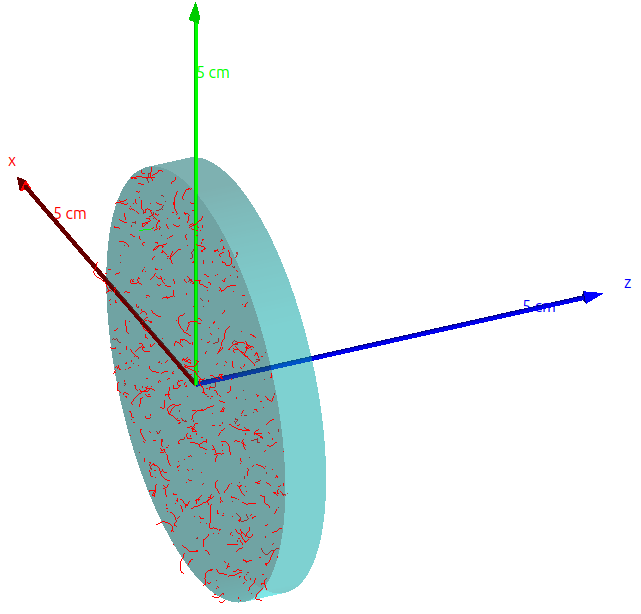
\includegraphics[width=0.5\textwidth]{figures/TritiumBetaPenetratePET.png}
	\caption{氚衰变 $\beta$ 穿透 PET 材料模型}
	\label{fig:TritiumBetaPenetratePET}
\end{figure}

氚衰变 $\beta$ 不经过膜窗,直接在氩气中沉积能量的能谱如图 \ref{fig:FullEdep} 所示。

\begin{figure}[htbp]
	\centering
	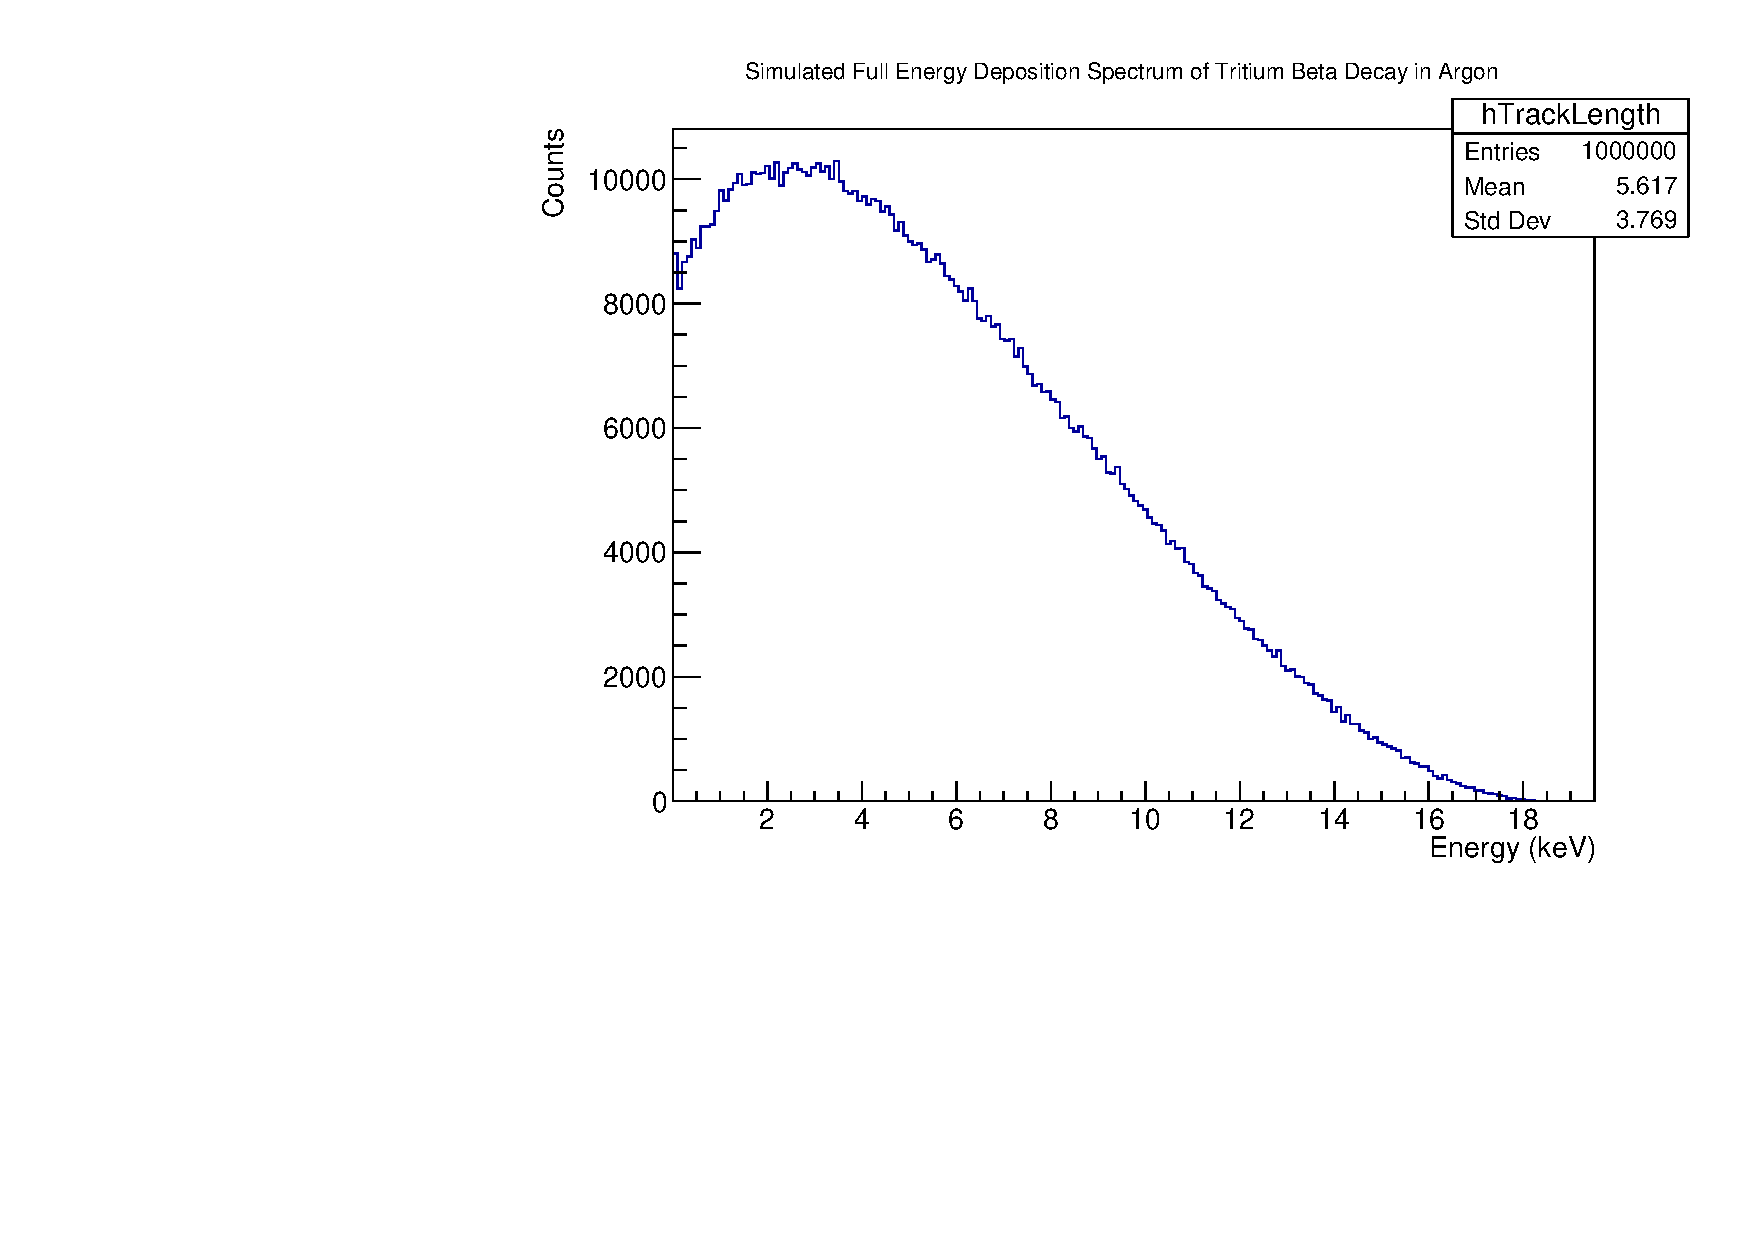
\includegraphics[width=0.6\textwidth]{figures/FullEdep.pdf}
	\caption{氚衰变 $\beta$ 在氩气中沉积能量的能谱}
	\label{fig:FullEdep}
\end{figure}

氚在氩气表面衰变时,在氩气中沉积能量的能谱如图 \ref{fig:0Edep} 所示。

氚衰变 $\beta$ 穿透了 \SI{0.1}{\micro\meter} 的 PET 材料,并在灵敏区沉积了能量,如图 \ref{fig:01Edep} 所示。

氚衰变 $\beta$ 穿透了 \SI{0.5}{\micro\meter} 的 PET 材料,并在灵敏区沉积了能量,如图 \ref{fig:05Edep} 所示。

氚衰变 $\beta$ 穿透了 \SI{1}{\micro\meter} 的 PET 材料,并在灵敏区沉积了能量,如图 \ref{fig:10Edep} 所示。

设置不同厚度的 PET 材料,模拟氚衰变 $\beta$ 穿透不同厚度的 PET 材料后在氩气中沉积事例占比,如图 \ref{fig:PETThickness} 所示。

\begin{figure}[htbp]
	\centering
	\begin{subfigure}[b]{0.45\textwidth}
		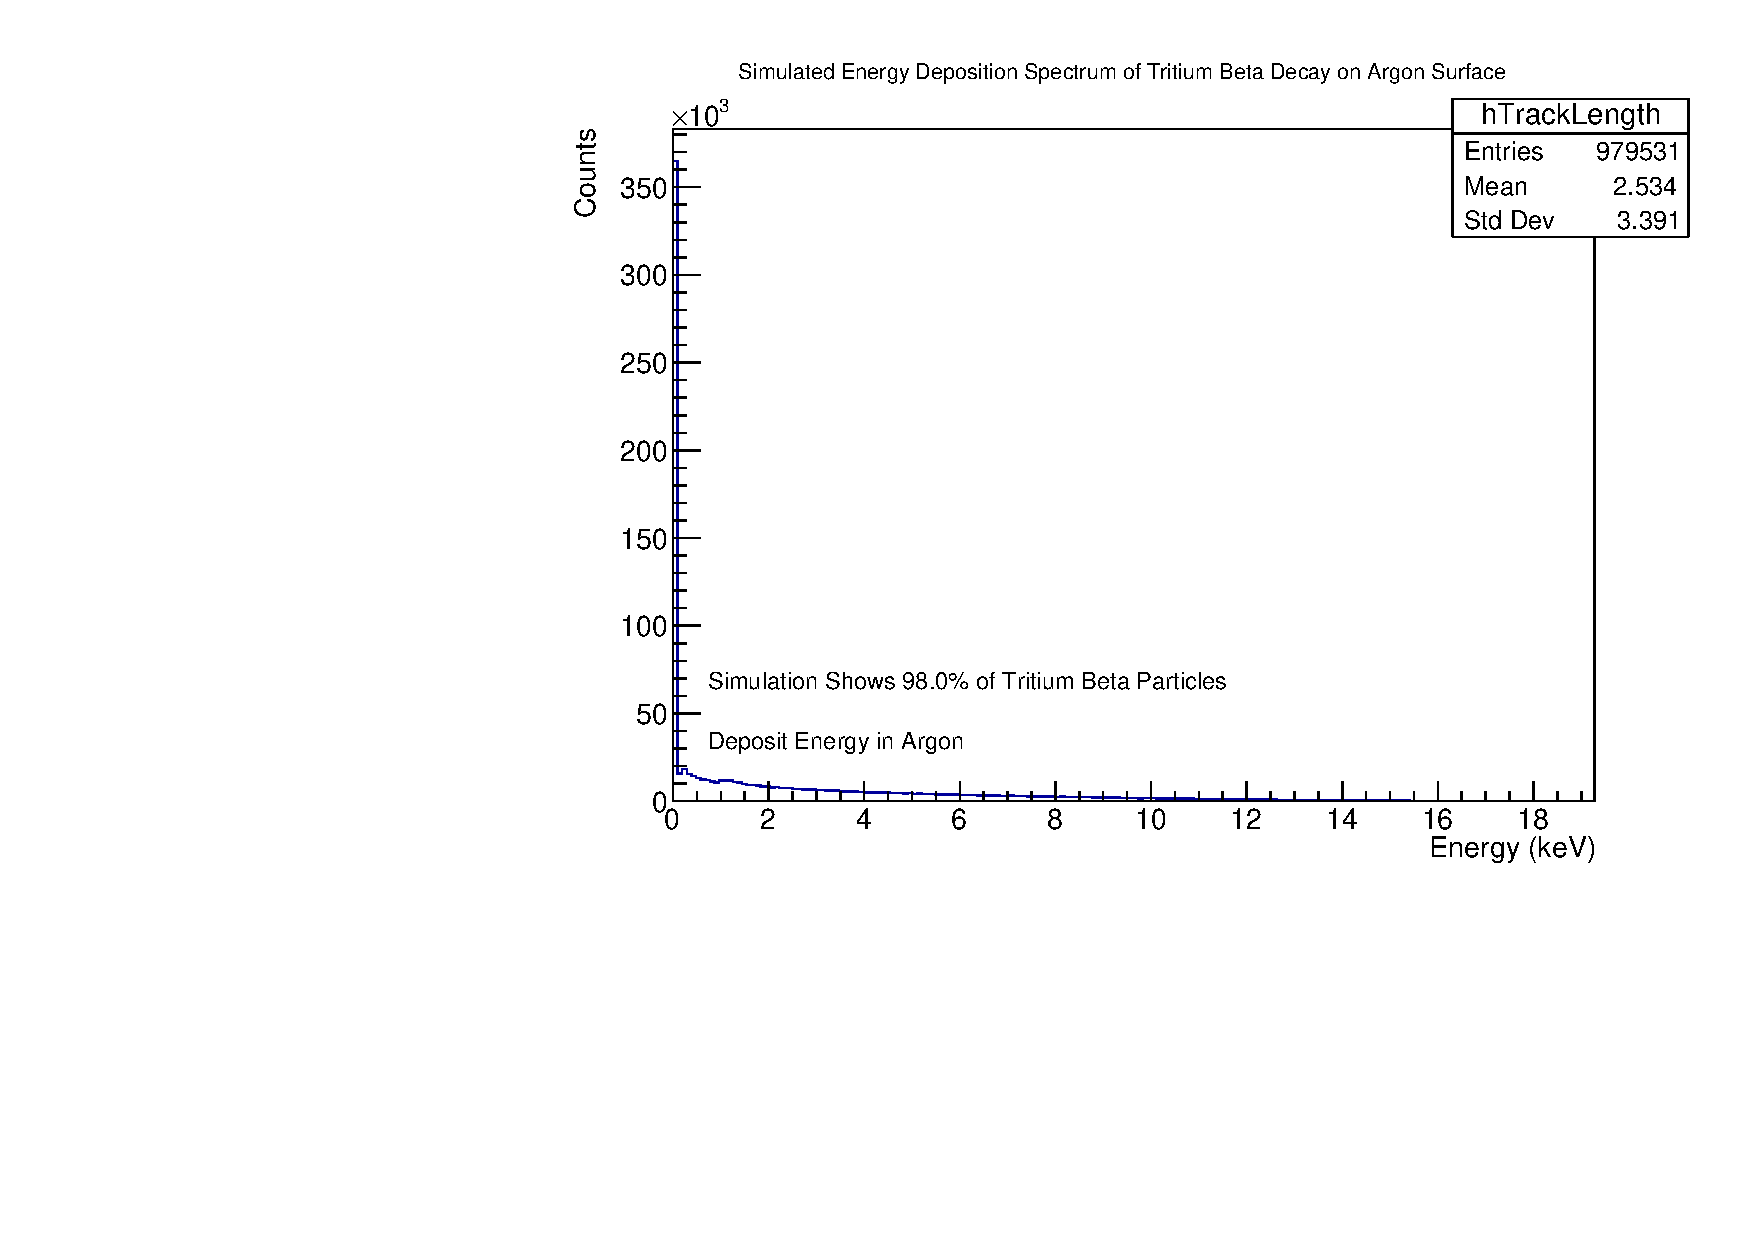
\includegraphics[width=\textwidth]{figures/0Edep.pdf}
		\caption{}
		\label{fig:0Edep}
	\end{subfigure}
	\hfill
	\begin{subfigure}[b]{0.45\textwidth}
		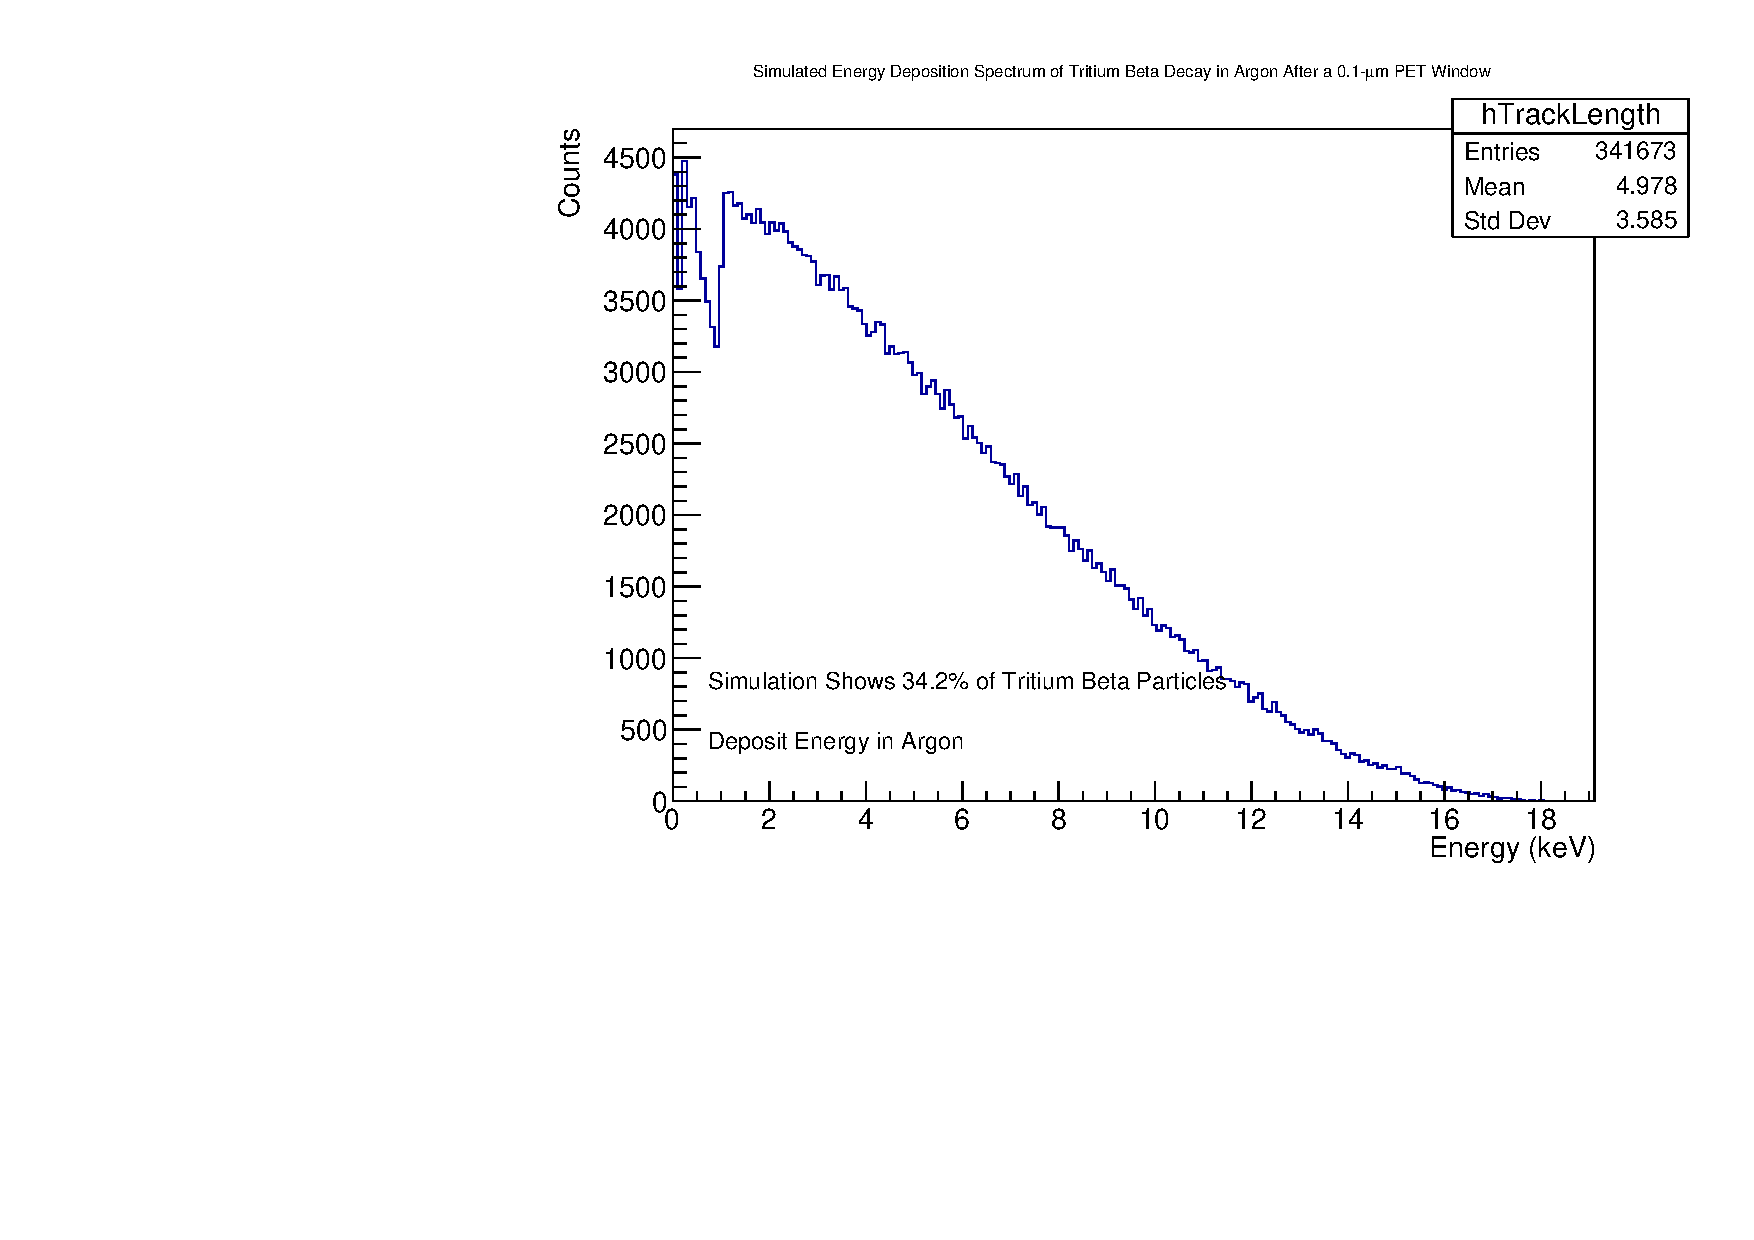
\includegraphics[width=\textwidth]{figures/01Edep.pdf}
		\caption{}
		\label{fig:01Edep}
	\end{subfigure}

	\begin{subfigure}[b]{0.45\textwidth}
		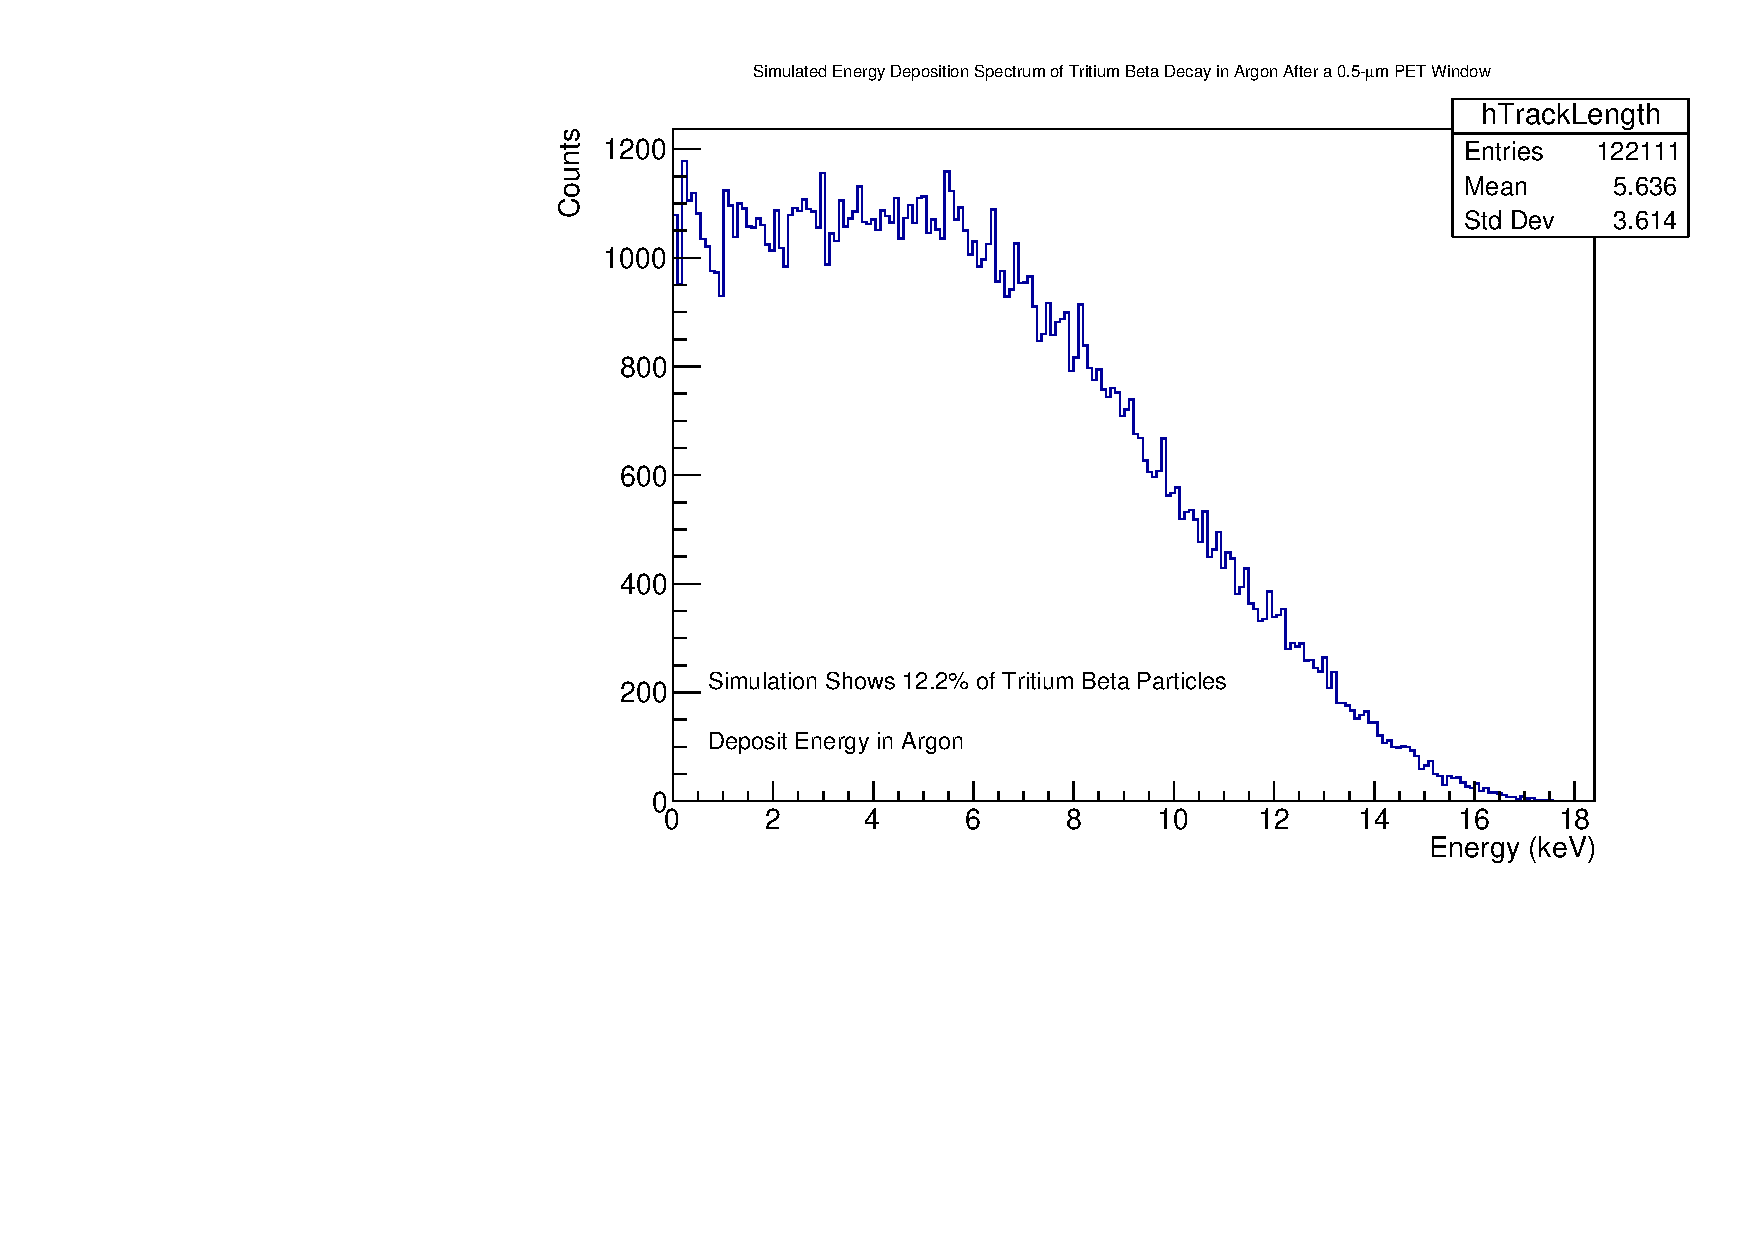
\includegraphics[width=\textwidth]{figures/05Edep.pdf}
		\caption{}
		\label{fig:05Edep}
	\end{subfigure}
	\hfill
	\begin{subfigure}[b]{0.45\textwidth}
		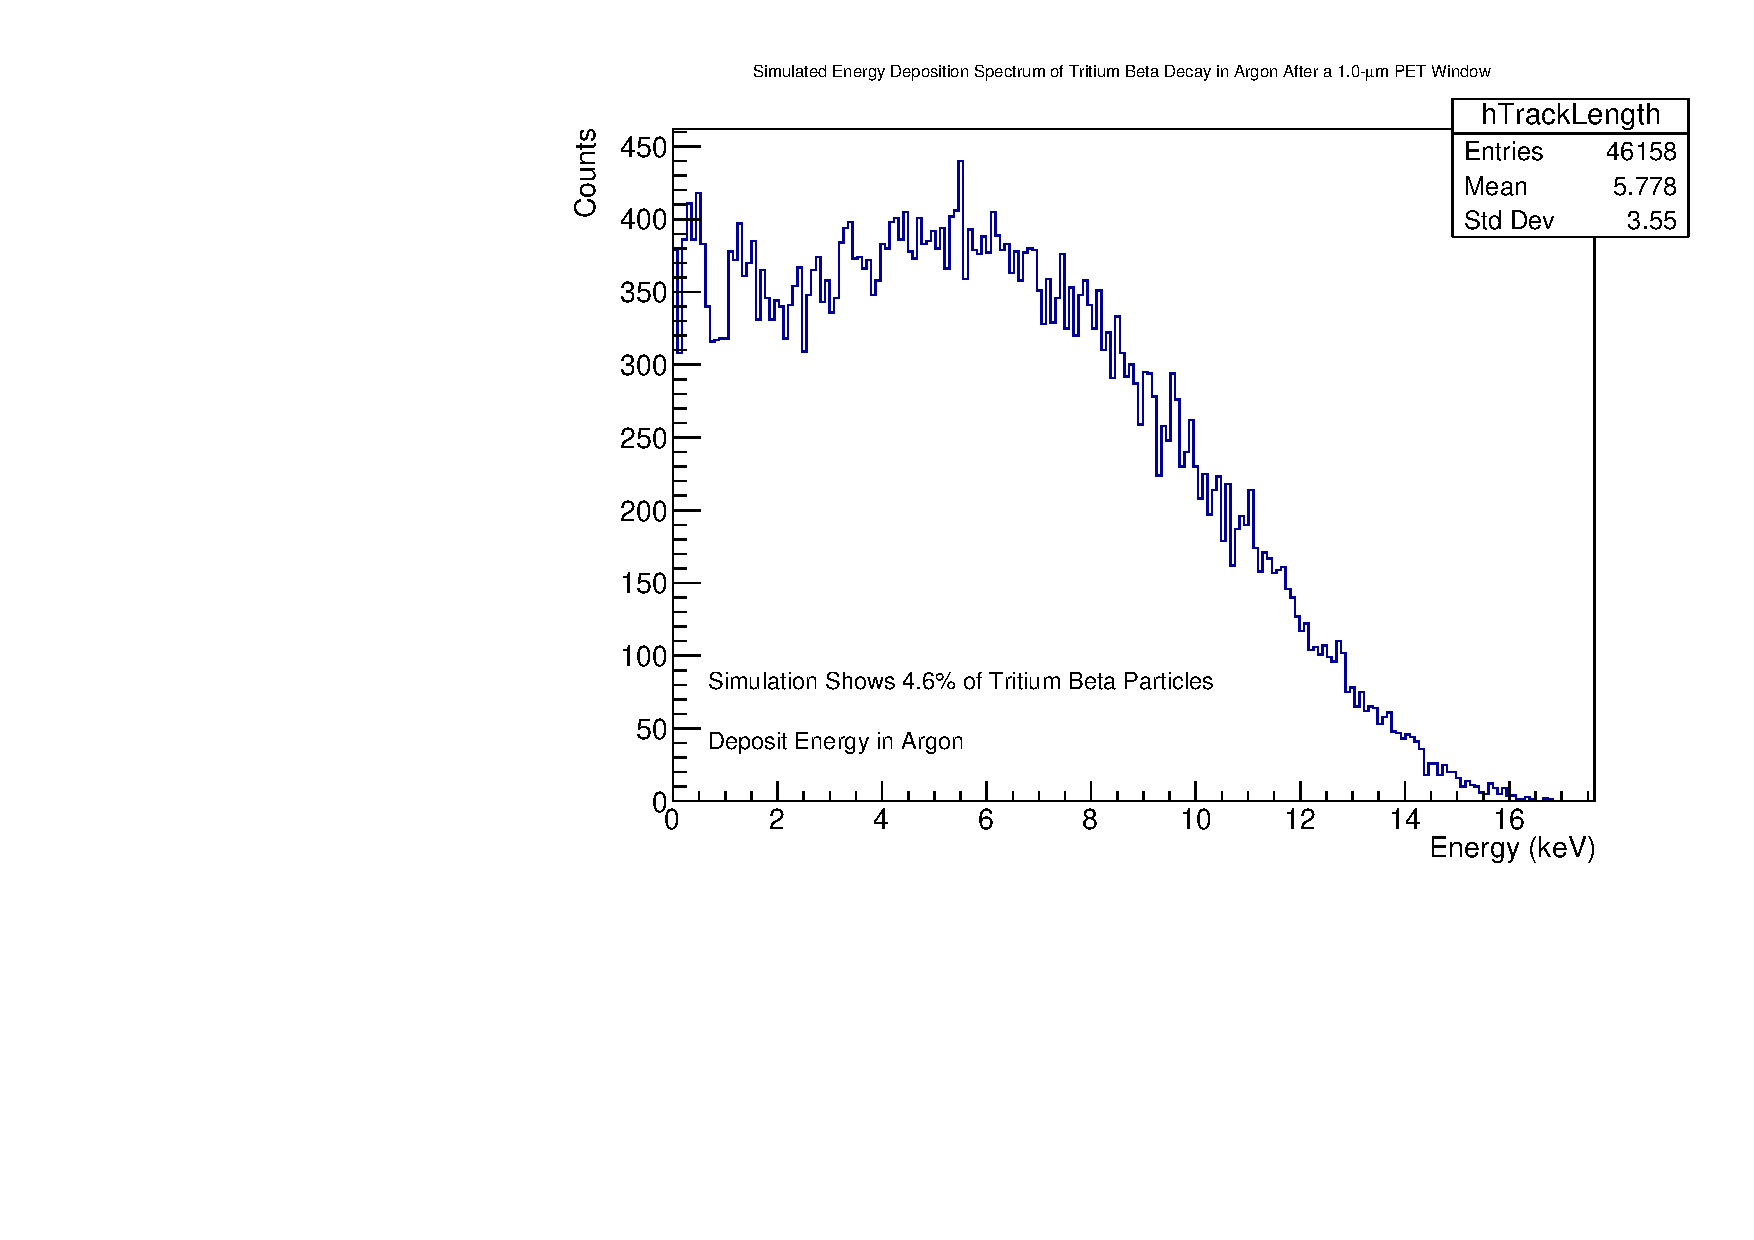
\includegraphics[width=\textwidth]{figures/10Edep.pdf}
		\caption{}
		\label{fig:10Edep}
	\end{subfigure}
	\caption{氚衰变 $\beta$ 穿透不同厚度的 PET 材料后在氩气中沉积的能谱。 (a) 在氩气表面衰变时,在氩气中沉积的能谱; (b) 穿透了 \SI{0.1}{\micro\meter} 的 PET 材料后在氩气中沉积的能谱; (c) 穿透了 \SI{0.5}{\micro\meter} 的 PET 材料后在氩气中沉积的能谱; (d) 穿透了 \SI{1}{\micro\meter} 的 PET 材料后在氩气中沉积的能谱}
	\label{fig:Edep}
\end{figure}

\begin{figure}[htbp]
	\centering
	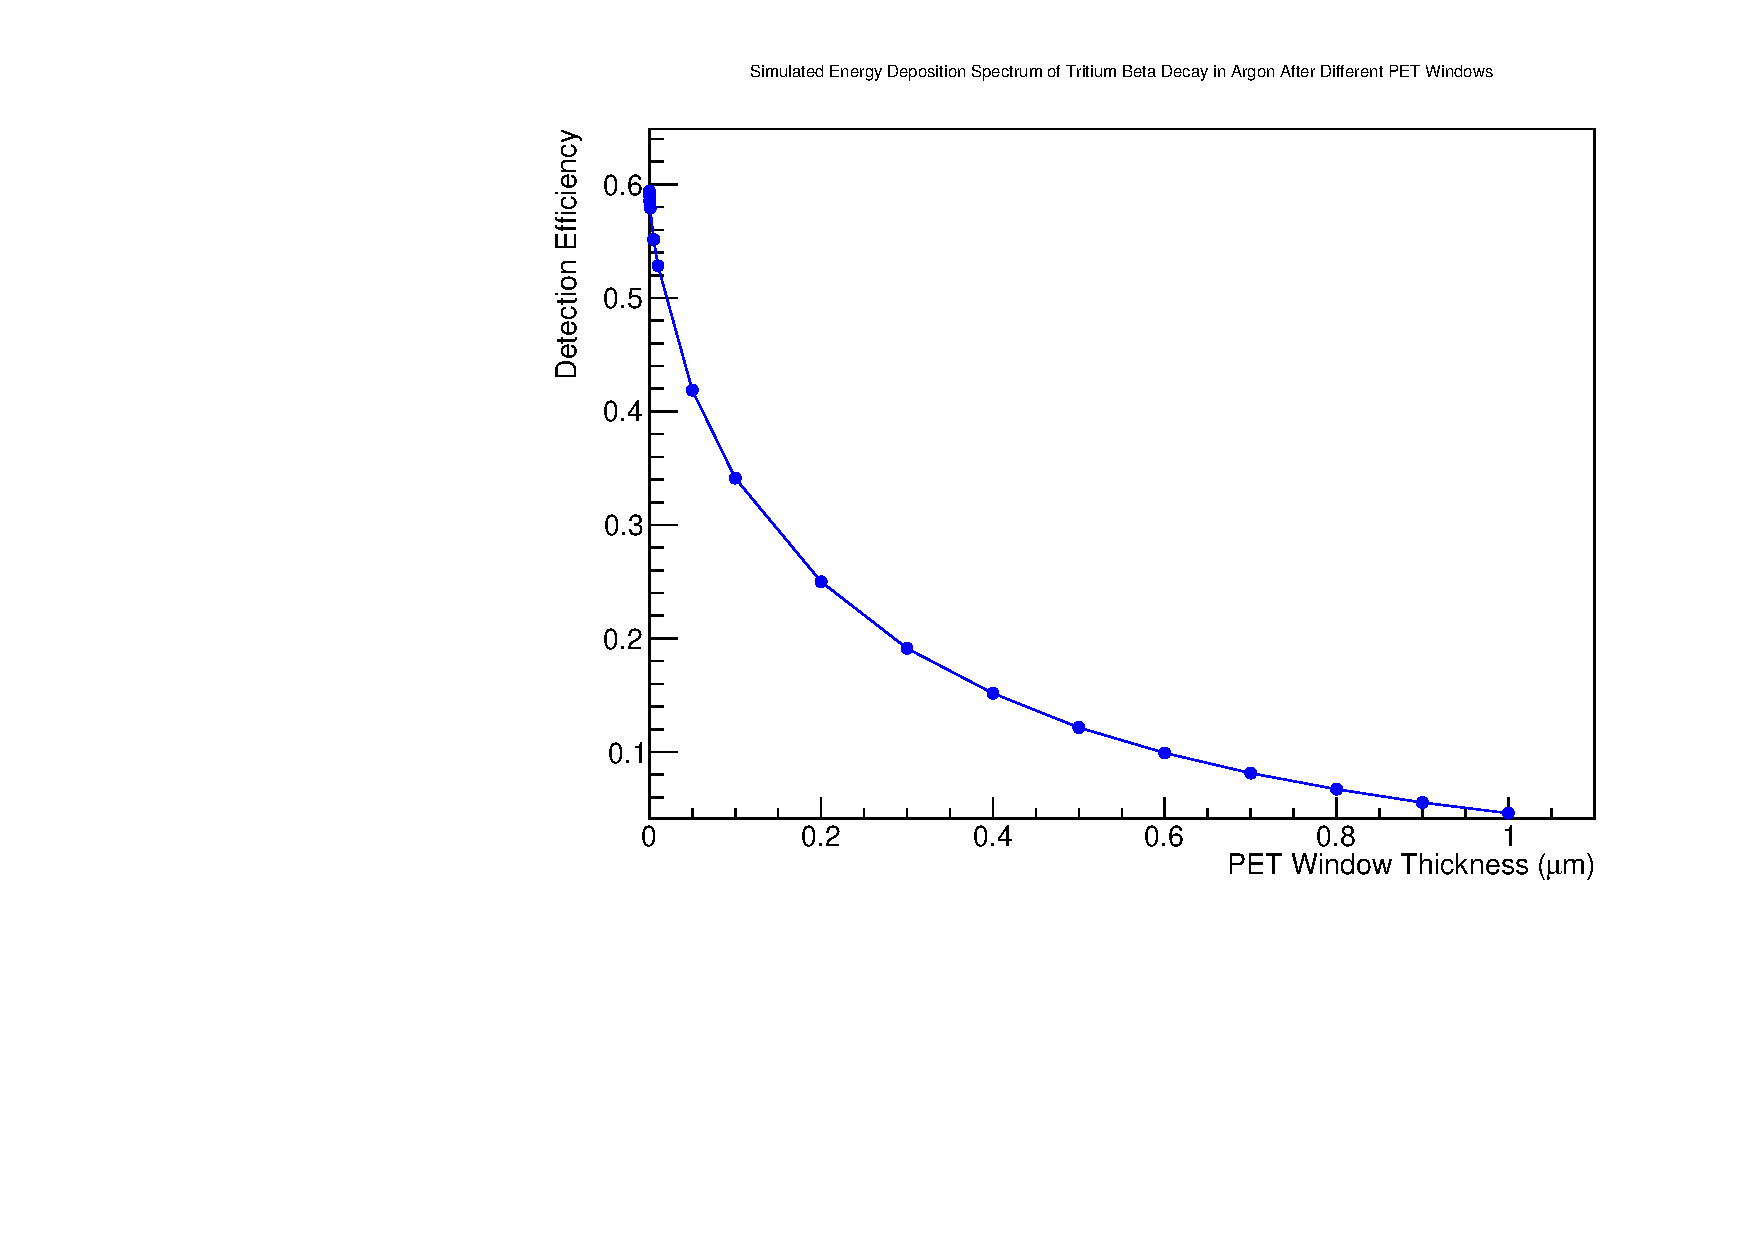
\includegraphics[width=0.8\textwidth]{figures/PETThickness.pdf}
	\caption{氚衰变 $\beta$ 穿透不同厚度的 PET 材料后在氩气中沉积事例占比}
	\label{fig:PETThickness}
\end{figure}

\begin{figure}[htbp]
	\centering
	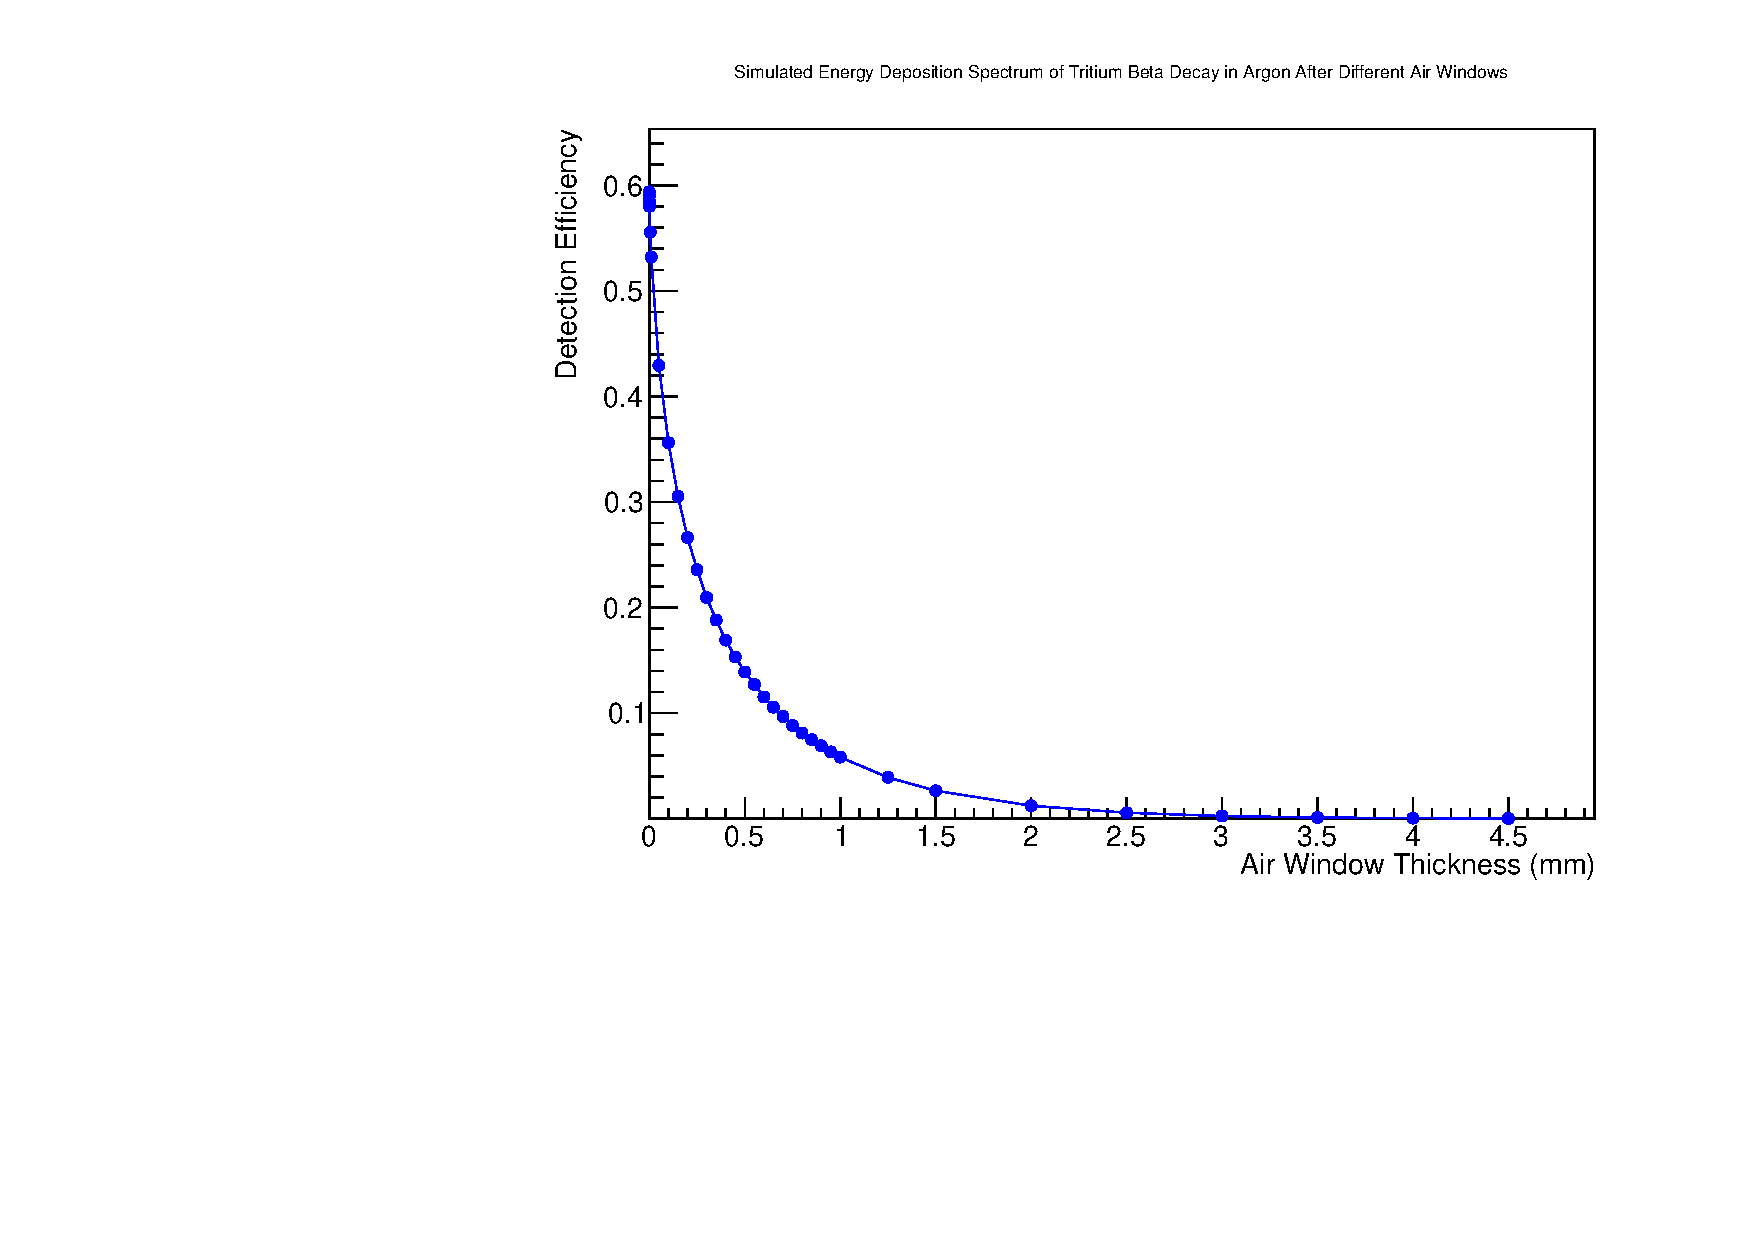
\includegraphics[width=0.8\textwidth]{figures/AirNEdep.pdf}
	\caption{氚衰变 $\beta$ 穿透不同厚度的 空气 后在氩气中沉积事例占比}
	\label{fig:AirThickness}
\end{figure}
